\label{sec:mmu}
Most processors strive to help the OS and its developers to ensure optimal
utilization of the main memory, as well as the overall security of the programs
memory usage.\\
In most systems, it is a common practice to split the memory into multiple
parts, where each part can only be accessed by the intended user. For example,
a user program should never be able to modify or even read memory of the kernel.
If that was possible, a single program would be able to break the running OS by
overwriting some essential values, or even retrieve passwords from variables in
other programs.\\
These mappings abstract the program addresses from the physical addresses, and
translation has to be implemented, to map these two address spaces. This is
usually done by the Memory Management Unit (MMU).\\
One of the big differences of the MIPS architecture is that many components in
the processor are completelly optional, and up for the manufacturer to decide
whether they suit the needs of the desired application, be it embedded device
or a supercomputer.\\
The memory management in MIPS32 is no exception, as MMU is completelly optional.
However, on MIPS32, to still ensure some basic form of user-restricted memory areas, the
memory is split into 4 areas, with each a designated
usage:\cite{imgtec:Memory_Map}\cite{see_mips_run}
\begin{itemize}
\item \textit{kseg0}, \texttt{0x80000000-0x9fffffff}, \texttt{512MiB}\\
The first kernel segment is which is translated by stripping of the first bit
in the address field. This segment is using caching, and can therefore first
be used when caches have been initiated.\cite{see_mips_run}
\item \textit{kseg1}, \texttt{0xa0000000-0xbfffffff}, \texttt{512MiB}\\
Kernel segment which is \textit{not} cached. It is the only segment that is
guaranteed to be available immediatelly after a system reset (or boot), where
no other CPU devices are initialized.
This is the segment where bootup-code is stored.
\item \textit{kuseg}, \texttt{0x00000000-0x7fffffff}, \texttt{2GiB}\\
This is the only segment that can be used by user programs. It is mapped and
cached, so the OS needs to initialize caches and possible MMU for this segment
to be useable.
\item \textit{kseg2}, \texttt{0xc0000000-0xffffffff}, \texttt{1GiB}\\
This segment is for additional access modes, such as the \textit{kernel}
mode. This segment is mapped and cached, and thus, cannot be used immediatelly after
bootup.
\end{itemize}

\subsection{Memory access privileges}
When the CPU starts up, it is by default in kernel mode. In this mode, it has
the privilege to access all addresses (along with many other things). The
kernel will retain this privilege until it starts user programs, in which case,
the OS flips the \texttt{KSU} bit in the co-processor0 status register\cite{harvard_mips_summary}.
Privilege levels are described in further detail in section
\ref{sec:privileges}.


\subsection{Implementation}
The simulator must support multiple memory sizes, for better simulation of
MIPS programs, as well as being more portable on host machines with limited
memory.\\
Since the physical addresses do not match the address of the data on the host
machine, an additional layer of memory mapping is created, which will ensure the
segment sizes still match. We will call these addresses for "actual" addresses,
representing the actual address on the host machine.\\
A new command-line flag "\texttt{-m}" followed by an integer is added to the
simulator, which will be used by the user to control how much actual memory is allocated
for the simulator memory. By default, this is 512MiB.\\
When the MMU module is initialized, the 4 segments are scaled accordingly --
\texttt{kuseg} is half of the allocated memory, \texttt{kseg2} makes up a quarter
of the memory and \texttt{kseg0} and \texttt{kseg1} share the rest.\\
Now that the addresses are allocated, the simulator needs a way to translate
between the layers of mappings.\\
All addresses an ordinary MIPS program uses, are virtual, that is, translated by
the processor. For translation of a virtual address, the simulator uses
\texttt{translate\_vaddr(uint32\_t vaddr)}, which translates an address to the
physical location on the simulated memory, or an IO device, discussed in section
\ref {sec:io}. However, since we are using a simulator, we must translate the
address further, into an "actual" address. For this, \texttt{translate\_paddr(uint32\_t paddr, ...)}
is used, which translates a physical address into an actual address -- the
address of the data on the host machine. A figure of an example mapping can be
seen on figure \ref{fig:address_space_mapping}.\\


\begin{figure*}[h]
	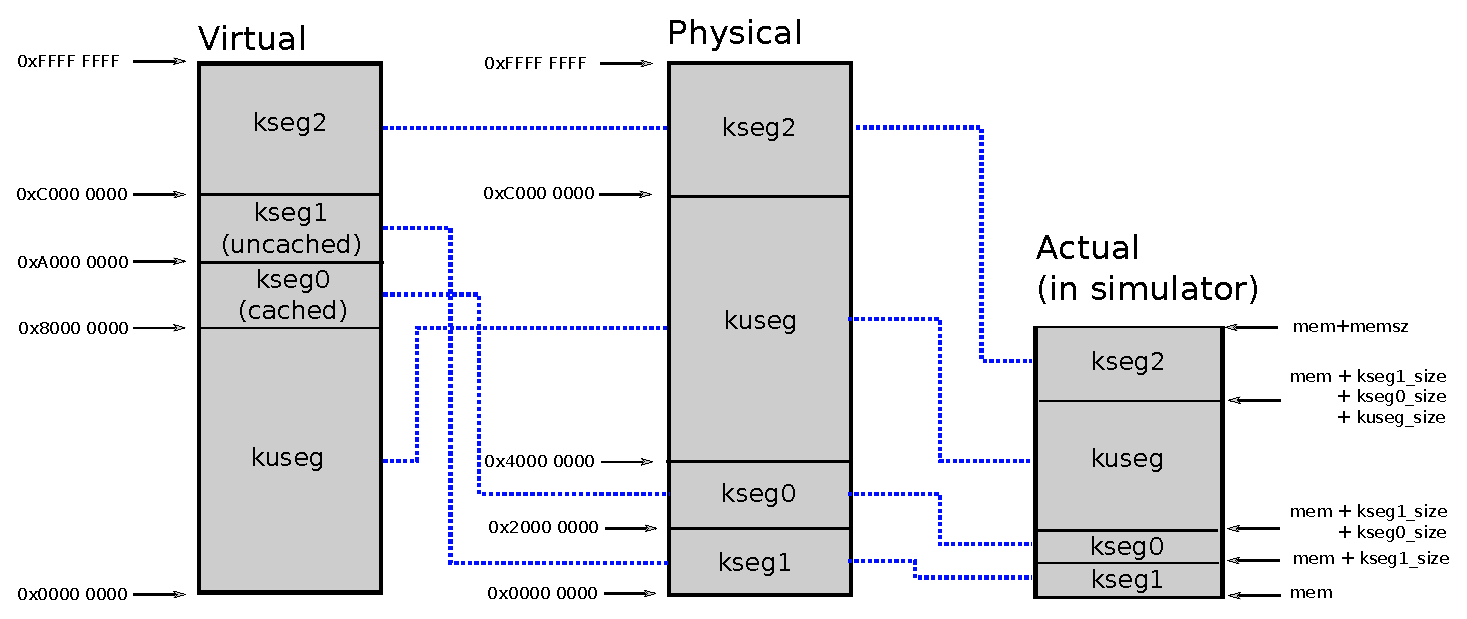
\includegraphics[width=\textwidth]{mmu/memory_mapping.eps}
	\caption{Main memory mapping in the simulator.}
	\label{fig:address_space_mapping}
\end{figure*}


